\chapter{Results}\label{ch:results}

This chapter reports what the validation apparatus of \cref{ch:validation} has
established. It is confined to correctness and coverage: how much of the
schedule-by-backend space is exercised, whether the backends agree, whether the
soundness gate behaves as designed, and how far the cluster and embedded tiers
have been confirmed. Performance --- compile time, generated-code size, runtime
scaling --- is out of scope for these results: the contribution this dissertation
defends is the separation and its falsifiability, not the speed of the emitted
code. Every number below is drawn from the live test apparatus.

\section{Coverage: examples, schedules, and backends}\label{sec:res-coverage}

The example corpus comprises twenty-seven worked algorithms, ranging from
elementwise addition and reduction through stencils, separable filters, matrix
multiplication, histogram, producer--consumer pipelines, a wavefront, the game of
life, bitonic sort, a small convolutional-network inference, a three-stage
hearing-aid pipeline, transpose, Jacobi iteration, sparse matrix--vector
multiplication, gather and scatter kernels, and a family of binned-combine
reductions. Each example carries one or more schedules expressing different
decompositions and IO disciplines, and the differential matrix declares, for each
schedule, the set of backends required to support it.

The full tier-1 matrix consists of \nmatrixtotal{} declared cells across the seven
shared-memory and message-passing CPU backends. Of these, \nmatrixpass{} pass ---
they emit, build, run, and reproduce the reference output byte-for-byte ---
\nmatrixskip{} are skipped for a stated reason, and none fail. The skipped cells are
not silent gaps: the matrix records a reason for every one, and they fall into a few
well-defined categories. The largest group, thirty-five cells, are embedded-tier fixtures
that are validated by the simulator gate of \cref{sec:res-tiers} rather than by the
tier-1 runtime rig, since the embedded backend emits \texttt{no\_std} code that the
hosted run-and-diff harness cannot execute. The remainder are genuine capability
mismatches --- an asynchronous, buffered schedule asked of a synchronous,
single-buffer backend, which is rejected at compile time as the capability matrix
prescribes (\cref{sec:be-matrix}) and whose required column is carried by a capable
sibling backend --- together with a small number of language shapes that are
honestly unsupported on the multi-worker path and documented as such
(\cref{sec:res-limits}). \Cref{fig:coverage-heatmap} renders the matrix as an
example-by-backend heatmap.

% fig:coverage-heatmap --- the tier-1 differential matrix as an example x backend
% heatmap. Cell status is the REAL per-(example,backend) status aggregated over
% schedules from nuc-nucleus/e2e-matrix.toml (P = all required cells pass; M =
% mixed, some schedule x backend cells skipped; s = all skipped). 26 examples
% appear in the tier-1 matrix (22-dma-pio-demo is embedded-only). Aggregate
% totals use the harness-verified macros. Grayscale-friendly (single-hue ramp).
\begin{figure}[tbp]
  \centering
  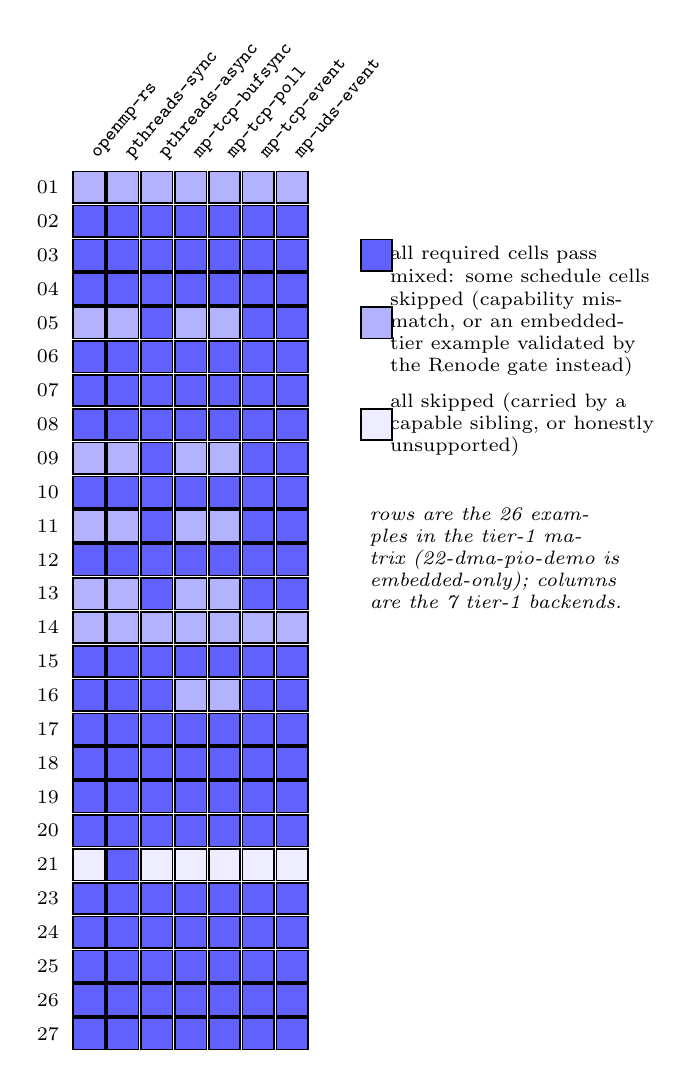
\begin{tikzpicture}[
      x=4.3mm, y=4.3mm,
      cell/.style={draw, semithick, minimum size=4.0mm, inner sep=0pt, anchor=center},
      P/.style={fill=blue!62}, M/.style={fill=blue!30}, s/.style={fill=blue!7},
    ]
    % backend column headers
    \foreach \be [count=\ci from 1] in {%
        openmp-rs, pthreads-sync, pthreads-async, mp-tcp-bufsync,
        mp-tcp-poll, mp-tcp-event, mp-uds-event}
      \node[rotate=50, anchor=west, font=\scriptsize\ttfamily] at (\ci, 0.7) {\be};
    % rows: example label + 7-cell status code (real data)
    \foreach \row/\lab [count=\ri from 0] in {%
        {M,M,M,M,M,M,M}/01, {P,P,P,P,P,P,P}/02, {P,P,P,P,P,P,P}/03,
        {P,P,P,P,P,P,P}/04, {M,M,P,M,M,P,P}/05, {P,P,P,P,P,P,P}/06,
        {P,P,P,P,P,P,P}/07, {P,P,P,P,P,P,P}/08, {M,M,P,M,M,P,P}/09,
        {P,P,P,P,P,P,P}/10, {M,M,P,M,M,P,P}/11, {P,P,P,P,P,P,P}/12,
        {M,M,P,M,M,P,P}/13, {M,M,M,M,M,M,M}/14, {P,P,P,P,P,P,P}/15,
        {P,P,P,M,M,P,P}/16, {P,P,P,P,P,P,P}/17, {P,P,P,P,P,P,P}/18,
        {P,P,P,P,P,P,P}/19, {P,P,P,P,P,P,P}/20, {s,P,s,s,s,s,s}/21,
        {P,P,P,P,P,P,P}/23, {P,P,P,P,P,P,P}/24, {P,P,P,P,P,P,P}/25,
        {P,P,P,P,P,P,P}/26, {P,P,P,P,P,P,P}/27} {
      \node[font=\scriptsize, anchor=east] at (0.4, -\ri) {\lab};
      \foreach \cell [count=\ci from 1] in \row
        \node[cell, \cell] at (\ci, -\ri) {};
    }
    % legend
    \node[cell, P, anchor=west] (lp) at (9.0, -2) {};
    \node[anchor=west, font=\scriptsize] at (9.6,-2) {all required cells pass};
    \node[cell, M, anchor=west] (lm) at (9.0, -4) {};
    \node[anchor=west, font=\scriptsize, align=left, text width=34mm] at (9.6,-4)
      {mixed: some schedule cells skipped (capability mismatch, or an
       embedded-tier example validated by the Renode gate instead)};
    \node[cell, s, anchor=west] (ls) at (9.0, -7) {};
    \node[anchor=west, font=\scriptsize, align=left, text width=34mm] at (9.6,-7)
      {all skipped (carried by a capable sibling, or honestly unsupported)};
    \node[anchor=west, font=\scriptsize\itshape, align=left, text width=34mm]
      at (9.0,-11) {rows are the 26 examples in the tier-1 matrix
      (22-dma-pio-demo is embedded-only); columns are the 7 tier-1 backends.};
  \end{tikzpicture}
  \caption[Tier-1 coverage heatmap]{The tier-1 differential matrix as an
    example-by-backend heatmap (rows are the 26 examples in the tier-1 matrix ---
    \texttt{22-dma-pio-demo} is embedded-only, hence the gap; columns are the
    seven tier-1 backends, of which \texttt{mp-uds-event} uses Unix-domain
    sockets). Each cell aggregates, over an example's schedules, its status on one
    backend: a dark cell (P) means every required schedule passes there, a mid
    cell (M) means some schedule is skipped, and a light cell (s) means all are
    skipped. Of \nmatrixtotal{} declared cells across the seven
    tier-1 backends, \nmatrixpass{} pass (emit, build, run, and reproduce the
    reference byte-for-byte), \nmatrixskip{} are skipped for a recorded reason ---
    the largest group embedded-tier fixtures validated by the simulator gate, the
    rest genuine capability mismatches carried by a capable sibling backend or a
    few honestly-unsupported language shapes --- and none fail. The broad band of
    dark cells is the cross-product of decompositions, IO disciplines, and
    runtimes exercised together on every build.}
  \label{fig:coverage-heatmap}
\end{figure}


The shape of this coverage is what gives the next section its force: it is not a
handful of examples on one backend, but a broad cross-product of decompositions,
IO disciplines, and runtimes, exercised together on every build.

\section{Bit-identity across the tier-1 matrix}\label{sec:res-bitidentity}

The central result is that the seven tier-1 backends agree byte-for-byte. Across
the \nmatrixpass{} passing cells, every backend required for a given example and
schedule reproduces that example's immutable reference output exactly, and the
backends are therefore byte-identical to one another, transitively, through that
shared reference. This holds uniformly across the diversity catalogued in
\cref{sec:val-differential}: the same algorithm under the same schedule produces the
same bytes whether its workers are threads sharing memory, processes exchanging
messages over TCP loopback, or processes over Unix-domain sockets; whether transfers
are synchronous or asynchronous, buffered or unbuffered; and whether the
notification discipline is a blocking receive, a non-blocking poll, or an event
reactor. The decomposition and IO machinery moves the same values to the same
places by the same final ordering, regardless of the runtime mechanism used to do
so. That is the genericity claim, and across the exercised matrix it is not
falsified.

One family of examples is worth singling out because it stresses the part of the
claim most likely to break under reordering. A distributed reduction that combines
per-worker partial results at a host accumulator is only order-independent if the
combining operation is associative and commutative; otherwise the order in which
workers arrive --- which legitimately varies across backends and runs --- would
change the result, and byte-identity would be lost. The system makes the combining
operation explicit --- declared as an attribute on the reducing kernel in the
algorithm (\cref{sec:lang-algorithm}) --- and supports six of them: integer sum,
bitwise or, bitwise xor, minimum, maximum, and bitwise and, each with its correct
algebraic identity element so that the accumulator is initialised soundly. Dedicated examples
exercise the non-trivial cases --- an xor-combined binned reduction, an
integer-minimum reduction whose identity is the type maximum rather than zero, and
the same in floating point. The discipline is enforced rather than assumed: a
floating-point \emph{sum} combine is \emph{rejected at compile time}, because
IEEE-754 addition is not associative and a distributed float-sum could not be made
byte-identical across arrival orders. Refusing the operation is more honest than
silently emitting code that happens to agree on the test input and diverges on
another.

\section{Soundness-gate outcomes}\label{sec:res-soundness}

The soundness gate runs on every build of every cell, so the matrix above is also a
record of the gate's behaviour on hundreds of real, shipping nets. On the committed
corpus the gate rejects nothing: every schedule that is supposed to be sound is
accepted, with no false rejections. This is the outcome a correct gate should
produce on a corpus of correct schedules, and on its own it would be weak evidence
--- an empty check produces the same green build. It is made meaningful by the
negative result alongside it. As described in \cref{sec:val-negative}, the gate's
three properties are each exercised adversarially by a unit test that hands it a
deliberately unsound net: an over-capacity net rejected as a boundedness error, a
stalling net rejected as a deadlock, and a free-choice net rejected as a conflict.
The gate accepts every sound net in the corpus \emph{and} is demonstrated capable
of rejecting unsound ones; both halves are necessary, and both hold. The harness's
own checks --- determinism, the cross-backend differential, and required-coverage
--- are guarded separately by the three injection falsifiers of
\cref{sec:val-negative}, so that no check in the pipeline, static or dynamic, is
trusted on its green result alone.

It bears repeating where the boundary of this result lies. The gate is sound for the
statically-ordered net class the language produces, by exact replay over one firing
order, and is not a general Petri-net model checker (\cref{sec:val-gate}). The
result is ``the gate correctly classifies the nets this system generates,'' not
``the gate decides boundedness for arbitrary nets,'' and the dissertation claims
only the former.

\section{Cluster and embedded value-correctness}\label{sec:res-tiers}

Beyond the tier-1 rig, the cluster and embedded tiers are confirmed to the extent
their runtimes allow, under the compile-mandatory, run-best-effort discipline of
\cref{sec:val-tiers}.

The two MPI backends compile for every schedule they are required to support and,
where a local \texttt{mpiexec} is available, are run and diffed against the same
reference files as the tier-1 backends. On that runtime every exercised MPI cell
reproduces its reference output byte-exactly: the single-program multiple-data
binary, dispatched across ranks, computes the same values as the shared-memory and
loopback backends. The blocking and non-blocking MPI backends thus extend the
byte-identity result from the laptop rig to a distributed-memory runtime, for the
cells exercised. The limit to be clear about is that this is value-correctness on a local
launcher, not a measurement on a production cluster, and that the backends emit
correct point-to-point communication rather than recognising and emitting
collective operations --- a deliberate deferral noted in \cref{sec:be-tier2}.

The embedded tier is confirmed by co-simulation. A standing gate generates the
bare-metal binaries for three multi-microcontroller examples, cross-compiles them
for the embedded target, co-simulates the microcontrollers wired over a virtual
UART fabric, captures the output bytes, and diffs them against the reference file.
All three reproduce their reference output byte-exactly: a two-microcontroller
split-and-add over a 1024-byte payload; the real three-core hearing-aid pipeline,
with heterogeneous front-end, DSP, and RF-controller workers and bidirectional
dataflow, over a 512-byte output; and a two-microcontroller demonstration that
drives two transfers by DMA and one by programmed IO over the same fabric,
again byte-exact over 1024 bytes. The hearing-aid result is the load-bearing one:
it demonstrates that the typed, heterogeneous, multi-worker form lowers all the way
to a real multi-microcontroller system whose per-frame values are correct
end-to-end, including the staged boot-order handling that a bare-metal UART channel
requires and that the hosted tiers never need.

\section{What the falsification rig establishes, and its limits}\label{sec:res-limits}

It is worth stating precisely what these results do and do not establish, because
the value of a falsification rig lies as much in the boundary of its claim as in the
claim itself.

What the rig establishes is this. For the exercised matrix --- twenty-seven
examples, their schedules, and the backends each requires --- the separation of
algorithm, schedule, and target holds to the strongest available standard:
byte-identical output across seven structurally diverse CPU runtimes, extended to a
distributed-memory MPI runtime and to bare-metal multi-microcontroller
co-simulation for the cells those tiers reach. The soundness gate correctly accepts
every sound schedule in the corpus and is demonstrated able to reject unsound nets.
Every check that underwrites these claims has a negative test proving it bites, so a
green result is informative rather than vacuous, and the whole apparatus is
reproducible from a pinned toolchain and a deterministic compiler.

What the rig does not establish is equally important. Byte-identity is shown over
the exercised cells, not proved for all programs the grammar admits; the
specification is exactly as complete as the example corpus, and a shape absent from
the corpus is outside the guarantee. Several such shapes are known and recorded
rather than hidden: a small number of cells are skipped because a language
construct is supported on the single-worker path but not yet on the multi-worker or
cross-backend path --- a data-dependent loop break, of the kind the language's
termination restriction already circumscribes (\cref{sec:lang-limits}), and a
worker-to-worker transfer nested inside a loop body --- and these are reported as
skips with a stated reason, not papered over. The cluster result is
value-correctness on a local launcher, not a cluster-scale measurement, and the MPI
backends emit point-to-point rather than collective communication. The embedded
result covers one reference microcontroller shim; further hardware families are
out-of-tree work. And, as the gate's design requires (\cref{sec:val-gate}), its
soundness guarantee is confined to the statically-ordered net class the
language produces.

The honest summary is that the falsification rig has had every opportunity to refute
the central claim over a broad and diverse matrix, and has not --- while the matrix's
documented edges mark exactly where the claim has not yet been put to the test.
That distinction, between what has survived falsification and what has not been
exposed to it, is the one this chapter is most concerned to keep clear.
